%%%%%%%%%%%%%%%%%%%%%%%%%%%%%%%%%%%%%%%%%
% Jacobs Landscape Poster
% LaTeX Template
% Version 1.1 (14/06/14)
%
% Created by:
% Computational Physics and Biophysics Group, Jacobs University
% https://teamwork.jacobs-university.de:8443/confluence/display/CoPandBiG/LaTeX+Poster
% 
% Further modified by:
% Nathaniel Johnston (nathaniel@njohnston.ca)
%
% This template has been downloaded from:
% http://www.LaTeXTemplates.com
%
% License:
% CC BY-NC-SA 3.0 (http://creativecommons.org/licenses/by-nc-sa/3.0/)
%
%%%%%%%%%%%%%%%%%%%%%%%%%%%%%%%%%%%%%%%%%

%----------------------------------------------------------------------------------------
%	PACKAGES AND OTHER DOCUMENT CONFIGURATIONS
%----------------------------------------------------------------------------------------

\documentclass[final]{beamer}

\usepackage[scale=1.24]{beamerposter} % Use the beamerposter package for laying out the poster
\setlength{\abovecaptionskip}{30pt plus 3pt minus 2pt}

%\captionsetup{width=0.8\textwidth}

\usepackage{fontawesome5}
\usepackage{natbib}

\usetheme{confposter} % Use the confposter theme supplied with this template

\setbeamercolor{block title}{fg=ngreen,bg=white} % Colors of the block titles
\setbeamercolor{block body}{fg=black,bg=white} % Colors of the body of blocks
\setbeamercolor{block alerted title}{fg=white,bg=dblue!70} % Colors of the highlighted block titles
\setbeamercolor{block alerted body}{fg=black,bg=dblue!10} % Colors of the body of highlighted blocks
% Many more colors are available for use in beamerthemeconfposter.sty

%-----------------------------------------------------------
% Define the column widths and overall poster size
% To set effective sepwid, onecolwid and twocolwid values, first choose how many columns you want and how much separation you want between columns
% In this template, the separation width chosen is 0.024 of the paper width and a 4-column layout
% onecolwid should therefore be (1-(# of columns+1)*sepwid)/# of columns e.g. (1-(4+1)*0.024)/4 = 0.22
% Set twocolwid to be (2*onecolwid)+sepwid = 0.464
% Set threecolwid to be (3*onecolwid)+2*sepwid = 0.708

\newlength{\sepwid}
\newlength{\onecolwid}
\newlength{\twocolwid}
\newlength{\threecolwid}
\setlength{\paperwidth}{48in} % A0 width: 46.8in
\setlength{\paperheight}{36in} % A0 height: 33.1in
\setlength{\sepwid}{0.024\paperwidth} % Separation width (white space) between columns
\setlength{\onecolwid}{0.22\paperwidth} % Width of one column
\setlength{\twocolwid}{0.464\paperwidth} % Width of two columns
\setlength{\threecolwid}{0.708\paperwidth} % Width of three columns
\setlength{\topmargin}{-0.5in} % Reduce the top margin size
%-----------------------------------------------------------

\usepackage{graphicx}  % Required for including images

\usepackage{booktabs} % Top and bottom rules for tables

\setbeamercolor{block title}{fg=black,bg=white} % Change the block title color


%----------------------------------------------------------------------------------------
%	TITLE SECTION 
%----------------------------------------------------------------------------------------


\title{BAIT: Benchmarking (Embedding) Architectures for Interactive Theorem-Proving} % Poster title

\author{
    Sean Lamont\textsuperscript{\rm 1,2},
    Michael Norrish\textsuperscript{\rm 1},
    Amir Dezfouli\textsuperscript{\rm 3},
    Christian Walder\textsuperscript{\rm 4},
    Paul Montague\textsuperscript{\rm 2}
}

\institute{
        \textsuperscript{\rm 1}Australian National University,
        \textsuperscript{\rm 2}Defence Science and Technology Group,
        \textsuperscript{\rm 3}BIMLOGIQ,
        \textsuperscript{\rm 4}Google DeepMind
    }



%----------------------------------------------------------------------------------------

\begin{document}

    \addtobeamertemplate{block end}{}{\vspace*{2ex}} % White space under blocks
    \addtobeamertemplate{block alerted end}{}{\vspace*{2ex}} % White space under highlighted (alert) blocks

    \setlength{\belowcaptionskip}{2ex} % White space under figures
    \setlength\belowdisplayshortskip{2ex} % White space under equations

    \begin{frame}[t] % The whole poster is enclosed in one beamer frame

        \begin{columns}[t] % The whole poster consists of three major columns,
%            the second of which is split into two columns twice - the [t] option aligns each column's content to the top

            \begin{column}{\sepwid}\end{column} % Empty spacer column

            \begin{column}{\onecolwid} % The first column

%----------------------------------------------------------------------------------------
%	OBJECTIVES
%----------------------------------------------------------------------------------------

                \begin{alertblock}{Summary}
                    We present BAIT, a platform to unify and \\ accelerate research in AI for Interactive Theorem-Proving (AI-ITP).
                    Using BAIT, we:

                    \begin{itemize}
                        \item Perform an in-depth comparison of modern embedding architectures over several Interactive Theorem Proving (ITP) benchmarks
                        \item Develop a novel End-to-End system for automated ITP,
                         outperforming previous work
                    \end{itemize}

                \end{alertblock}

%----------------------------------------------------------------------------------------
%	INTRODUCTION
%----------------------------------------------------------------------------------------

                \begin{block}{Motivation}
                    \begin{itemize}
                        \item ITP systems are essential to formal verification
                        \item Broad applications, from pure mathematics to critical software
                        \item ITP applications typically require expert human guidance, limiting their scalability
                        \item Recent work in AI-ITP has shown promise in applying AI to automate and assist ITP guidance
                        \item AI-ITP results are fragmented, with many different approaches spread across several ITPs
                        \item In particular, the Embedding architectures used across AI-ITP approaches have not been compared thoroughly
                    \end{itemize}

                \end{block}

                \begin{block}{BAIT}

                    \begin{itemize}
                        \item Implements the setup in Figure~\ref{aitp},
                        which represents many AI-ITP approaches
                        \item A modular design decouples the
                        Search, Model, Environment and Data
                        \item Shared checkpointing, logging and experiment management
                        \item Streamlines the integration and comparison of
                        components, with minimal boilerplate
                        \item Facilitates reproducibility and transparency
                    \end{itemize}

                \end{block}


%------------------------------------------------


%----------------------------------------------------------------------------------------

            \end{column} % End of the first column

            \begin{column}{\sepwid}\end{column} % Empty spacer column

            \begin{column}{\twocolwid} % Begin a column which is two columns wide (column 2)

                \begin{columns}[t,totalwidth=\twocolwid] % Split up the two columns wide column

                    \begin{column}{\onecolwid}
                        \vspace{-.6in} % The first column within column 2 (column 2.1)

%----------------------------------------------------------------------------------------
%	MATERIALS
%----------------------------------------------------------------------------------------

                        \begin{block}{AI-ITP Setup}
                            \begin{figure}
                                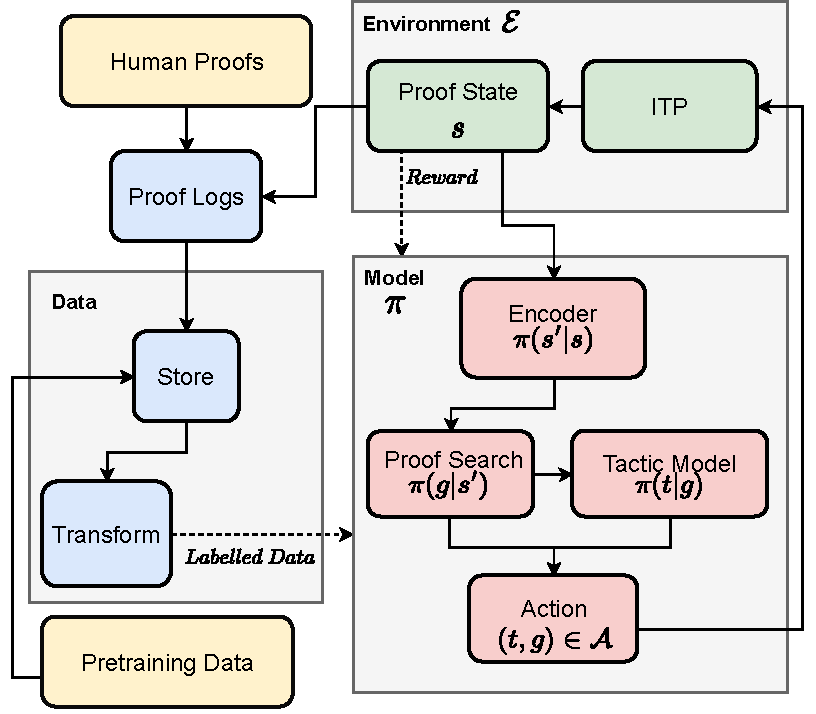
\includegraphics[width=\linewidth]{aitp}
                                \caption{ AI-ITP setup.
                                A model $\pi$ interacts with a proving environment $\mathcal{E}$,
                                    mapping a state $s$ to an action $(t,g)$, which defines tactic(s) $t$ to apply to goal(s) $g \subseteq s$.
                                    $\pi$ is trained with rewards or Data from processed Proof Logs, based on human proofs or agent-environment interactions.
                                    Implementing this modular framework, BAIT streamlines the integration and comparison of different approaches and benchmarks.}
                            \end{figure}
                            \label{aitp}
                        \end{block}


%----------------------------------------------------------------------------------------

                    \end{column} % End of column 2.1

                    \begin{column}{\onecolwid}
                        \vspace{-.6in} % The second column within column 2 (column 2.2)

%----------------------------------------------------------------------------------------
%	METHODS
%----------------------------------------------------------------------------------------


                        \begin{block}{Experiments}

                            \begin{table}[h]
                                \centering
                                \begin{tabular}{lcc}
                                    \toprule
                                    Model               & Cumulative      & pass@1          \\
                                    \midrule
                                    GNN (Ours)          & 96.2\%          & \textbf{64.6\%} \\
                                    Transformer (Ours)  & \textbf{96.8\%} & 63.3\%          \\
                                    Original TacticZero & 90.7\%          & 43.0\%          \\
                                    \bottomrule
                                \end{tabular}
                                \caption{ Goals proven by TacticZero~\cite{wu_tacticzero_2021} in HOL4, after 1 attempt for validation and cumulatively for training.
                                Experiments with the Embedding architecture result in large performance gains compared to the original.}
                                \label{fig:tz_plotfirst}
                            \end{table}%

                            Our experiments are over two categories:

                            \begin{itemize}
                                \item Supervised, with the task of predicting the tactic or premise used in a proof step.
                                We compare Structure Aware Transformers (SAT)~\cite{chen_structure-aware_2022, luo_transformers_2023},
                                Graph Neural Networks (GNNs)~\cite{wang_premise_2017}, Transformer Encoders~\cite{vaswani_attention_2017} and an Ensemble of GNN + Transformer over seven supervised ITP datasets
                                \item End-to-End, where the agent interacts with a live environment and learns from self-play.
                                We use the SoTA TacticZero~\cite{wu_tacticzero_2021} agent, with the associated HOL4 environment, and compare its original Encoder to GNN and Transformer Encoders
                            \end{itemize}


                        \end{block}

%----------------------------------------------------------------------------------------

                    \end{column} % End of column 2.2

                \end{columns} % End of the split of column 2 - any content after this will now take up 2 columns width

%----------------------------------------------------------------------------------------
%	IMPORTANT RESULT
%----------------------------------------------------------------------------------------
                \begin{block}{Embedding Comparison}

                    \renewcommand{\arraystretch}{1.5}
                    \begin{table}[h]
                        \centering
                        \begin{tabular}[t]{lcr}
                            \toprule
                            Expression & GNN Encoder (Our Approach) & Original TacticZero \\
                            \midrule
                            $\mathsf{diag}(A) = \mathsf{diag}(A^T)$ &
                            $R = (R^T)^T$ &
                            $\mathsf{FINITE}(\mathsf{POW}(s)) \Leftrightarrow \mathsf{FINITE}(s)$ \\
                            %
                            $R\;x\; y \Rightarrow \mathsf{RC}(R)\; x\; y$ &
                            $\mathsf{RC}(\mathsf{RC}(R)) = \mathsf{RC}(R)$ &
                            $R \;x \;y \Rightarrow \mathsf{EQC}(R)\;x \;y$  \\
                            %
                            $s \subseteq t \Leftrightarrow s \cup t = t$ &
                            $ s\; \mathsf{DIFF}\; t = \emptyset \Leftrightarrow s \subseteq t$&
                            $\mathsf{SURJ}\; f\; s\; t \Leftrightarrow \mathsf{IMAGE}\; f\; s = t$\\
                            $ s \cup t = t \cup s$ &
                            $ s \cup (t \cup u) = (s \cup t) \cup u$ &
                            $s \cap t = t \cap s$ \\
                            %
                            $ (s \cup t) x \Leftrightarrow x \in s
                            \lor x \in t$ &
                            $x \in s \cup t \;\Leftrightarrow\; x \in s \lor x \in t$ &
                            $ (s \cap t) x \Leftrightarrow x \in s \land x \in t$ \\
                            \bottomrule
                        \end{tabular}
                        \caption{ A selection of mathematical expressions (left) along with the nearest expression by cosine distance according to the \alg{TacticZero} encoder (right) and our GNN encoder (center).
                        Note the nearest neighbor as
                        judged by the GNN model is generally far more semantically relevant to
                        the original expression than the nearest neighbor as
                        judged by the original TacticZero~\cite{wu_tacticzero_2021} Autoencoder.
                        }
                        \label{fig:qual1}
                    \end{table}%



                \end{block}{}

%----------------------------------------------------------------------------------------

            \end{column} % End of the second column

            \begin{column}{\sepwid}\end{column} % Empty spacer column

            \begin{column}{\onecolwid} % The third column

%----------------------------------------------------------------------------------------
%	CONCLUSION
%----------------------------------------------------------------------------------------

                \begin{alertblock}{Results}
                    \begin{itemize}
                        \item For supervised benchmarks, SAT~\cite{chen_structure-aware_2022, luo_transformers_2023},
                        and Ensemble methods improve upon GNN~\cite{wang_premise_2017} and Transformer Encoder~\cite{vaswani_attention_2017} models,
                        with SAT models performing the best overall.
                        \item  We reveal a significant improvement in the SoTA TacticZero~\cite{wu_tacticzero_2021}
                        through experiments with the Embedding architecture (Table~\ref{fig:tz_plotfirst}).
                        We observed this was associated with more semantically relevant embeddings (Table~\ref{fig:qual1})
                    \end{itemize}
                \end{alertblock}


%----------------------------------------------------------------------------------------
%	REFERENCES
%----------------------------------------------------------------------------------------

                \begin{block}{References}
                    \small{\bibliographystyle{unsrt}
                    \bibliography{ref}\vspace{0.75in}}

                    \setbeamercolor{block alerted title}{fg=black,bg=norange} % Change the alert block title colors
                    \setbeamercolor{block alerted body}{fg=black,bg=white} % Change the alert block body colors

                    \begin{alertblock}{Links}

                        \begin{itemize}
                            \item \faLink : \href{https://sean-lamont.github.io/bait}{sean-lamont.github.io/bait}
                            \item \faGithub : \href{https://github.com/sean-lamont/bait}{github.com/sean-lamont/bait}
                            \item \faEnvelope : \href{mailto:sean.a.lamont@outlook.com}{sean.a.lamont@outlook.com}
                        \end{itemize}

                    \end{alertblock}


                \end{block}

%----------------------------------------------------------------------------------------
%	CONTACT INFORMATION
%----------------------------------------------------------------------------------------



%----------------------------------------------------------------------------------------
%	ACKNOWLEDGEMENTS
%----------------------------------------------------------------------------------------

%                \setbeamercolor{block title}{fg=red,bg=white} % Change the block title color

                \begin{block}{Acknowledgements}

                    \small{\rmfamily{
                        We would like to acknowledge Defence Science and Technology Group (DSTG) for their support in this project.
                        We would also like to thank Minchao Wu for his help with the TacticZero source code.
                    }} \\
                \end{block}


%----------------------------------------------------------------------------------------

            \end{column} % End of the third column

        \end{columns} % End of all the columns in the poster

    \end{frame} % End of the enclosing frame

\end{document}
